% ============================================================
%  CHAPTER: VILA-Style Embodied AI Agent for TIAGo
%  Generated from project source — /home/lissi/tiago_public_ws
% ============================================================

\documentclass[12pt,a4paper]{report}

% ---- Packages -----------------------------------------------
\usepackage[utf8]{inputenc}
\usepackage[T1]{fontenc}
\usepackage[english]{babel}
\usepackage{geometry}
\geometry{left=2.5cm,right=2.5cm,top=2.5cm,bottom=2.5cm}

\usepackage{graphicx}
\usepackage{amsmath}
\usepackage{amssymb}
\usepackage{booktabs}
\usepackage{longtable}
\usepackage{array}
\usepackage{tabularx}
\usepackage{multirow}
\usepackage{xcolor}
\usepackage{listings}
\usepackage{caption}
\usepackage{subcaption}
\usepackage{hyperref}
\usepackage{tikz}
\usepackage{pgf-umlsd}
\usepackage{enumitem}
\usepackage{fancyhdr}
\usepackage{setspace}
\usepackage{mdframed}
\usepackage{float}
\usepackage[ruled,vlined]{algorithm2e}

\usetikzlibrary{shapes.geometric, arrows, positioning, fit, calc, decorations.pathreplacing}

% ---- Colours ------------------------------------------------
\definecolor{darkblue}{RGB}{0,51,102}
\definecolor{lightblue}{RGB}{173,216,230}
\definecolor{codegray}{RGB}{245,245,245}
\definecolor{codegreen}{RGB}{0,128,0}
\definecolor{codepurple}{RGB}{128,0,128}
\definecolor{codered}{RGB}{180,0,0}
\definecolor{palgreen}{RGB}{0,160,80}

% ---- Code listings ------------------------------------------
\lstset{
  backgroundcolor=\color{codegray},
  commentstyle=\color{codegreen},
  keywordstyle=\color{darkblue}\bfseries,
  stringstyle=\color{codered},
  basicstyle=\ttfamily\small,
  breakatwhitespace=false,
  breaklines=true,
  captionpos=b,
  keepspaces=true,
  numbers=left,
  numbersep=8pt,
  numberstyle=\tiny\color{gray},
  showspaces=false,
  showstringspaces=false,
  showtabs=false,
  tabsize=2,
  frame=single,
  rulecolor=\color{gray!40},
  xleftmargin=15pt,
}

\lstdefinelanguage{JSON}{
  morestring=[b]",
  literate=
   *{:}{{{\color{darkblue}{:}}}}{1}
    {,}{{{\color{darkblue}{,}}}}{1}
    {\{}{{{\color{darkblue}{\{}}}}{1}
    {\}}{{{\color{darkblue}{\}}}}}{1}
    {[}{{{\color{darkblue}{[}}}}{1}
    {]}{{{\color{darkblue}{]}}}}{1}
}

% ---- Header / Footer ----------------------------------------
\pagestyle{fancy}
\fancyhf{}
\rhead{\small VILA Embodied AI Agent — TIAGo Robot}
\lhead{\small Technical Report}
\rfoot{\thepage}

% ---- Hyperref -----------------------------------------------
\hypersetup{
  colorlinks=true,
  linkcolor=darkblue,
  urlcolor=darkblue,
  citecolor=darkblue,
  pdftitle={VILA-Style Embodied AI Agent for TIAGo},
  pdfauthor={Technical Report},
}

% ============================================================
\begin{document}
% ============================================================

% ---- Title Page --------------------------------------------
\begin{titlepage}
  \centering
  \vspace*{2cm}
  {\Huge\bfseries\color{darkblue}
    VILA-Style Embodied AI Agent\\[0.4em]
    for the TIAGo Mobile Manipulator
  \par}
  \vspace{1cm}
  \rule{\linewidth}{1.5pt}
  \vspace{0.5cm}
  {\large\itshape
    A Vision--Language--Action System Integrating\\
    Gemini 2.0 Flash, YOLO11n, and ROS Melodic\\
    for Natural-Language-Driven Manipulation Tasks
  \par}
  \vspace{0.5cm}
  \rule{\linewidth}{0.8pt}
  \vspace{2cm}

  \begin{tabular}{ll}
    \textbf{Platform}  & PAL Robotics TIAGo (ROS Melodic, Docker) \\
    \textbf{VLM}       & Google Gemini 2.0 Flash REST API \\
    \textbf{Detector}  & YOLO11n via HTTP microservice (Python 3.10 host) \\
    \textbf{Interface} & Voice (Whisper STT) + Text + PAL TTS \\
    \textbf{Date}      & \today \\
  \end{tabular}

  \vfill
  {\small Technical Report — Project Documentation Series}
\end{titlepage}

% ---- Table of Contents -------------------------------------
\tableofcontents
\clearpage

% ============================================================
\chapter{Introduction and Motivation}
% ============================================================

\section{Problem Statement}

Mobile manipulation robots such as PAL Robotics' TIAGo offer a versatile hardware platform
for domestic and industrial service tasks.  Despite their physical capabilities, programming
these robots for complex, multi-step tasks has traditionally required explicit, hand-crafted
skill sequences.  A user wishing the robot to \emph{``find the bottle and bring it to me''}
would previously need a hard-coded state machine that cannot generalise to variations in
object position, lighting, or scene context.

This report describes the design and implementation of a \textbf{Vision--Language--Action
(VLA) agent} for TIAGo that bridges natural-language commands, visual perception, and
physical skill execution.  Inspired by the SayCan \cite{saycancite} and VILA \cite{vilacite}
families of embodied AI, the system enables the robot to:

\begin{itemize}[noitemsep]
  \item Understand voice or text commands in natural language,
  \item Observe the environment through its RGB-D camera,
  \item Reason about which action to take using a multimodal large language model (VLM),
  \item Execute modular manipulation skills, and
  \item Recover safely from failures without human intervention.
\end{itemize}

\section{Scope}

The deployment environment is a single-room laboratory scenario.  Target tasks include:

\begin{enumerate}[noitemsep]
  \item Grasping a bottle from a table,
  \item Handing the bottle to a nearby person,
  \item Searching for an object by scanning with the head,
  \item Returning the arm to a safe home posture.
\end{enumerate}

Navigation between pre-defined named locations (table, shelf, handover spot) is supported
via the ROS move\_base / Nav2 stack, though the current deployment focuses on the
manipulation pipeline.

% ============================================================
\chapter{System Architecture}
% ============================================================

\section{High-Level Architecture}

The agent follows a \textbf{perceive–reason–act} loop as illustrated in
Figure~\ref{fig:arch}.  At each iteration:

\begin{enumerate}
  \item The robot captures an RGB image from its Asus Xtion (RGBD) sensor.
  \item YOLO11n detects objects and returns bounding boxes with class names and
        confidence scores.
  \item The current robot state (gripper status, task history, detected objects) is
        assembled by the \texttt{StateManager}.
  \item A prompt combining the image, detections, state, and user command is sent to
        \textbf{Google Gemini 2.0 Flash} via its REST API.
  \item The VLM returns a JSON response nominating a \emph{skill} to execute next,
        together with parameters and a natural-language rationale.
  \item The nominated skill's \emph{affordance check} verifies that preconditions are met.
  \item The skill executes and updates the state.
  \item The loop repeats until the VLM reports the task is complete, a maximum step
        count is reached, or a safety condition is triggered.
\end{enumerate}

% --- Architecture Diagram ---
\begin{figure}[H]
\centering
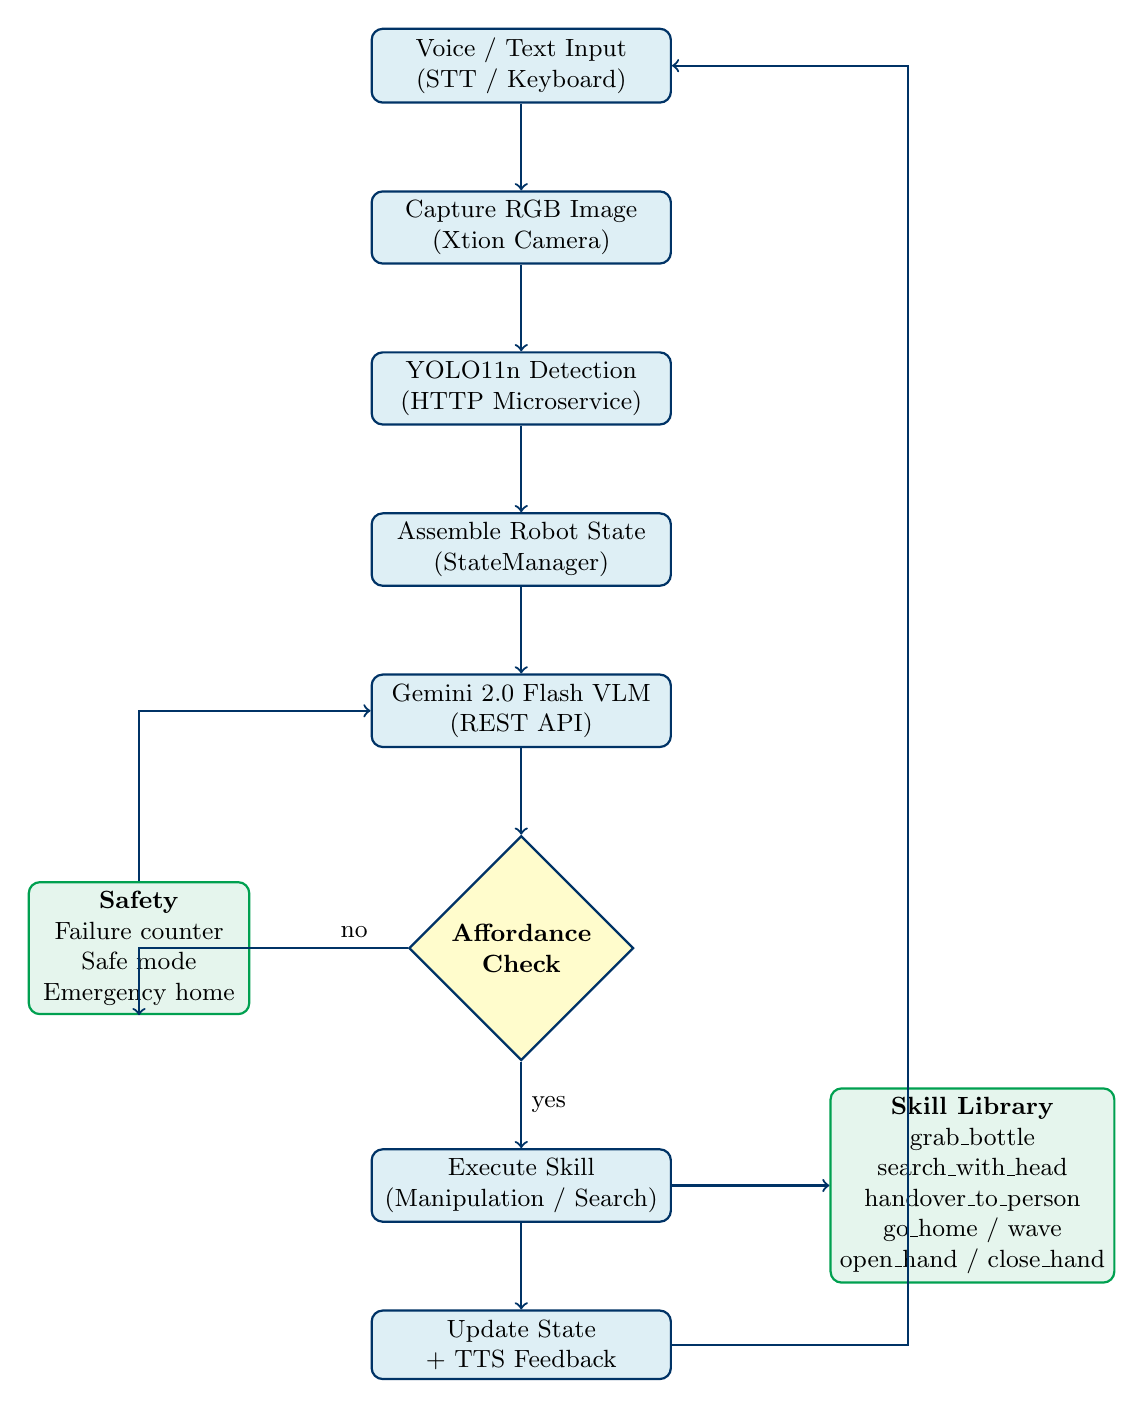
\begin{tikzpicture}[
  node distance=1.1cm and 1.8cm,
  box/.style={rectangle, rounded corners=4pt, draw=darkblue, thick,
              fill=lightblue!40, minimum width=3.8cm, minimum height=0.85cm,
              align=center, font=\small},
  decision/.style={diamond, draw=darkblue, thick, fill=yellow!20,
                   minimum width=2cm, minimum height=0.8cm, align=center, font=\small\bfseries},
  arr/.style={->, thick, draw=darkblue},
  side/.style={rectangle, rounded corners=4pt, draw=palgreen, thick,
               fill=palgreen!10, minimum width=2.8cm, minimum height=0.75cm,
               align=center, font=\small},
]
  % Main flow (vertical)
  \node[box] (voice)   {Voice / Text Input\\(STT / Keyboard)};
  \node[box, below=of voice]  (percept){Capture RGB Image\\(Xtion Camera)};
  \node[box, below=of percept](yolo)   {YOLO11n Detection\\(HTTP Microservice)};
  \node[box, below=of yolo]   (state)  {Assemble Robot State\\(StateManager)};
  \node[box, below=of state]  (vlm)    {Gemini 2.0 Flash VLM\\(REST API)};
  \node[decision, below=of vlm](afford){Affordance\\Check};
  \node[box, below=of afford] (exec)   {Execute Skill\\(Manipulation / Search)};
  \node[box, below=of exec]   (update) {Update State\\+ TTS Feedback};

  % Skill side panel
  \node[side, right=2cm of exec] (skills){
    \textbf{Skill Library}\\
    grab\_bottle\\
    search\_with\_head\\
    handover\_to\_person\\
    go\_home / wave\\
    open\_hand / close\_hand
  };

  % Safety side
  \node[side, left=2cm of afford] (safety){
    \textbf{Safety}\\
    Failure counter\\
    Safe mode\\
    Emergency home
  };

  % Arrows
  \draw[arr] (voice)   -- (percept);
  \draw[arr] (percept) -- (yolo);
  \draw[arr] (yolo)    -- (state);
  \draw[arr] (state)   -- (vlm);
  \draw[arr] (vlm)     -- (afford);
  \draw[arr] (afford)  -- node[right]{\small yes} (exec);
  \draw[arr] (exec)    -- (update);
  \draw[arr] (exec)    -- (skills);

  % Affordance fail → back to VLM
  \draw[arr] (afford.west) -| (safety.south)
      node[pos=0.1, above]{\small no};
  \draw[arr] (safety.north) |- (vlm.west);

  % Loop back
  \draw[arr] (update.east) -| ([xshift=3cm]update.east)
      |- ([xshift=3cm]voice.east) -- (voice.east);

\end{tikzpicture}
\caption{High-level architecture of the VILA Embodied AI Agent.}
\label{fig:arch}
\end{figure}

\section{Deployment Architecture}

A key constraint of the TIAGo robot is that its onboard software stack runs inside a
\textbf{Docker container} (image \texttt{reverent\_einstein}) using
\textbf{Python 3.6} and \textbf{ROS Melodic}.  Modern deep learning libraries (Ultralytics
YOLO $\geq$ 8, PyTorch $\geq$ 2.x) require Python $\geq$ 3.8 and are therefore
\emph{incompatible} with the container environment.

The solution adopted is a \textbf{split-process architecture}:

\begin{center}
\begin{tabular}{lll}
\toprule
\textbf{Component} & \textbf{Process} & \textbf{Python / OS} \\
\midrule
Embodied Agent (control loop) & Docker container & Python 3.6 / ROS Melodic \\
Perception Manager v2         & Docker container & Python 3.6 / ROS Melodic \\
VLM Reasoner (Gemini client)  & Docker container & Python 3.6 \\
YOLO Service (\texttt{yolo\_service.py}) & Host machine   & Python 3.10 / Ubuntu 22 \\
Live Detector stream           & Docker container & Python 3.6 \\
\bottomrule
\end{tabular}
\end{center}

The Docker container uses \texttt{--network host}, which means both processes share
\texttt{localhost}.  The YOLO service listens on port \textbf{5001}; the live MJPEG
visualiser on port \textbf{8081}.

% ============================================================
\chapter{Technologies Used}
% ============================================================

\section{Hardware Platform}

\subsection{PAL Robotics TIAGo}

TIAGo is a mobile manipulator featuring:

\begin{itemize}[noitemsep]
  \item \textbf{Mobile base:} Omnidirectional wheels with laser odometry.
  \item \textbf{Torso lift:} Single prismatic joint (0--35 cm stroke).
  \item \textbf{Arm:} 7-DOF (shoulder yaw, shoulder pitch, shoulder roll, elbow, wrist yaw, wrist pitch, wrist roll).
  \item \textbf{Gripper:} PAL parallel two-finger gripper.
  \item \textbf{Head:} 2-DOF pan--tilt (\texttt{head\_1\_joint} for pan, \texttt{head\_2\_joint} for tilt).
  \item \textbf{Sensor:} Asus Xtion Pro Live (RGB-D) at 640$\times$480, registered depth aligned to RGB.
  \item \textbf{Microphone:} USB audio capture for speech input.
\end{itemize}

\section{Middleware: ROS Melodic}

The Robot Operating System (ROS) Melodic (Ubuntu 18.04 base) provides the communication
backbone:

\begin{description}[noitemsep]
  \item[\texttt{/xtion/rgb/image\_raw}] Raw BGR/RGB camera stream (sensor\_msgs/Image).
  \item[\texttt{/xtion/depth\_registered/image\_raw}] Depth aligned to RGB (32FC1 or 16UC1).
  \item[\texttt{/xtion/rgb/camera\_info}] Camera intrinsics for 3-D projection.
  \item[\texttt{/joint\_states}] Continuous joint position stream (used for gripper state and head pan preservation).
  \item[\texttt{/mobile\_base\_controller/odom}] Wheel odometry for base pose tracking.
  \item[\texttt{/play\_motion}] PAL \texttt{play\_motion} action server for pre-defined arm trajectories.
  \item[\texttt{/move\_group}] MoveIt action server for Cartesian/joint-space arm planning.
  \item[\texttt{/tts}] PAL TTS action server (pal\_interaction\_msgs/TtsAction).
  \item[\texttt{/head\_controller/follow\_joint\_trajectory}] Head trajectory controller.
  \item[\texttt{/torso\_controller/follow\_joint\_trajectory}] Torso trajectory controller.
  \item[\texttt{/agent/camera\_annotated}] Agent-published annotated image for live visualiser.
  \item[\texttt{/agent/status}] JSON status string for the web dashboard.
\end{description}

\section{Object Detection: YOLO11n}

Object detection is performed by \textbf{Ultralytics YOLO11n} (nano variant), the
fastest model in the YOLO11 family, selected for its real-time inference at $<$25 ms
on CPU.  The model is trained on the MS-COCO 80-class dataset, covering all objects
relevant to the deployment scenario (\texttt{bottle}, \texttt{person}, \texttt{cup},
\texttt{chair}, etc.).

\subsection{YOLO HTTP Microservice}

Because the Docker container runs Python 3.6, YOLO11n is deployed on the host machine
as a standalone HTTP service (\texttt{yolo\_service.py}):

\begin{lstlisting}[language=Python, caption={YOLO service — inference endpoint (excerpt).}]
class _Handler(BaseHTTPRequestHandler):
    def do_POST(self):
        jpeg_bytes = self.rfile.read(int(self.headers['Content-Length']))

        # Optional per-request class override via header
        classes_header = self.headers.get('X-Classes', '')
        classes = [c.strip() for c in classes_header.split(',') if c.strip()] \
            if classes_header else None

        detections = _run_inference(jpeg_bytes, classes=classes)
        # Returns: [{"class_name": str, "confidence": float, "bbox": [x,y,w,h]}, ...]
\end{lstlisting}

\subsubsection{API Contract}

\begin{center}
\begin{tabularx}{\linewidth}{llX}
\toprule
\textbf{Method} & \textbf{Endpoint} & \textbf{Description} \\
\midrule
POST & \texttt{/detect} & Body: raw JPEG bytes. Header \texttt{X-Classes}: comma-separated class names for filtering. Returns JSON detections. \\
GET  & \texttt{/health} & Returns model name, open-vocab flag, segmentation flag. \\
\bottomrule
\end{tabularx}
\end{center}

\subsubsection{Detection Response Format}

\begin{lstlisting}[language=JSON, caption={Detection JSON response schema.}]
{
  "detections": [
    {
      "class_name": "bottle",
      "confidence": 0.8712,
      "bbox": [142, 201, 85, 178]
    },
    {
      "class_name": "person",
      "confidence": 0.9341,
      "bbox": [310, 120, 200, 380]
    }
  ],
  "model": "yolo11n",
  "inference_ms": 18,
  "segmentation": false
}
\end{lstlisting}

\subsection{Live YOLO Visualiser}

A separate script (\texttt{live\_detector.py}) runs in the Docker container and provides
a browser-accessible MJPEG stream at \texttt{http://localhost:8081} showing real-time
YOLO detections overlaid on the camera feed.  It uses a \textbf{decoupled two-thread
architecture} to avoid stream jitter:

\begin{itemize}[noitemsep]
  \item \textbf{Camera thread:} Reads raw frames from \texttt{/xtion/rgb/image\_raw} and
        composites the \emph{last known} detection boxes at 15 fps.
  \item \textbf{Detection thread:} Calls the YOLO service independently as fast as possible
        (typically 8--15 Hz for YOLO11n), updating the shared detection list.
\end{itemize}

This ensures the stream remains smooth even when detection is slower than the camera rate.

\section{Vision--Language Model: Google Gemini 2.0 Flash}

The reasoning backbone is \textbf{Google Gemini 2.0 Flash}, accessed via the
\textbf{Google Generative Language REST API}.  Key properties relevant to the deployment:

\begin{center}
\begin{tabular}{ll}
\toprule
\textbf{Property} & \textbf{Value} \\
\midrule
Modality          & Text + Image (multimodal) \\
Context window    & 1M tokens \\
Input pricing     & $\approx$\$0.10 per 1M tokens \\
Output pricing    & $\approx$\$0.40 per 1M tokens \\
Typical latency   & 0.4--1.0 s per call \\
Image encoding    & JPEG, Base64 inline \\
API endpoint      & \texttt{generativelanguage.googleapis.com/v1beta} \\
\bottomrule
\end{tabular}
\end{center}

Gemini was chosen over alternatives (Groq llama-3.2-vision, GPT-4o) because:

\begin{itemize}[noitemsep]
  \item Native multimodal understanding with \emph{grounded} spatial reasoning.
  \item Stable, well-documented REST API compatible with Python 3.6 (\texttt{requests} library only).
  \item Competitive cost for image-heavy workloads ($\approx$\$0.005 per image at 640$\times$480 JPEG).
  \item 1 M-token context allows full task history with embedded images.
\end{itemize}

\section{Speech Recognition and Synthesis}

\subsection{Speech-to-Text (STT)}

The agent supports two STT backends with automatic fallback:

\begin{enumerate}[noitemsep]
  \item \textbf{OpenAI Whisper (local, ``base'' model)} via \texttt{speech\_recognition}
        library.  Preferred because it runs offline and handles accented English well.
  \item \textbf{Google Cloud STT} via \texttt{recognize\_google()}.  Used as fallback
        when Whisper fails or is unavailable.
\end{enumerate}

Microphone selection is automatic: the agent prefers USB audio interfaces, then
the HDA Intel PCH ALC codec, then the system default.  When PulseAudio is detected
(typical in Docker with X11 forwarding), the default audio device is used to avoid
ALSA conflicts.

\subsection{Text-to-Speech (TTS)}

Speech output uses the \textbf{PAL TTS action server} (\texttt{/tts},
\texttt{pal\_interaction\_msgs/TtsAction}) with British English (\texttt{en\_GB}).
The agent speaks short, human-readable status phrases at each step
(``Looking at the scene.'', ``Executing grab bottle.'', ``Task complete!'').

\section{Arm Planning: MoveIt}

Three-dimensional arm motion is planned by the \textbf{MoveIt motion planning framework}
via the \texttt{/move\_group} action server.  Planning uses the \texttt{arm\_torso} planning
group (arm + torso lift joint), OMPL as the default planner, and the following parameters
for robust execution:

\begin{center}
\begin{tabular}{ll}
\toprule
\textbf{Parameter} & \textbf{Value} \\
\midrule
Planning attempts  & 10 \\
Allowed planning time & 12 s \\
Max velocity scaling & 0.3 \\
Max acceleration scaling & 0.2 \\
Replan attempts    & 3 \\
\bottomrule
\end{tabular}
\end{center}

Position constraints are expressed as spheres (radius 5--8 cm) around target Cartesian
positions in the \texttt{base\_footprint} frame.  A soft orientation constraint
($\pm$0.4 rad tolerance on all axes) preserves the gripper orientation during handover.

% ============================================================
\chapter{Software Components}
% ============================================================

\section{Component Overview}

\begin{center}
\begin{tabularx}{\linewidth}{lXl}
\toprule
\textbf{File} & \textbf{Role} & \textbf{Lines} \\
\midrule
\texttt{embodied\_agent\_v2.py}  & Main control loop, STT/TTS, safety orchestration & $\approx$664 \\
\texttt{vlm\_reasoner.py}        & Gemini REST client, prompt builder, image encoder & $\approx$370 \\
\texttt{perception\_manager\_v2.py} & RGB capture + YOLO service client, fallback DNN & $\approx$230 \\
\texttt{state\_manager.py}       & Robot state tracking, scene graph, spatial relations & $\approx$380 \\
\texttt{yolo\_service.py}        & Host-side YOLO11n HTTP microservice & $\approx$220 \\
\texttt{live\_detector.py}       & MJPEG live stream with decoupled detection & $\approx$280 \\
\texttt{reach\_object\_v5\_torso\_descent\_working.py} & Full bottle grasp pipeline & $\approx$700 \\
\texttt{skills/base\_skill.py}   & Abstract base class for skills & $\approx$80 \\
\texttt{skills/grab\_bottle.py}  & Grasp skill (calls reach\_object via subprocess) & $\approx$140 \\
\texttt{skills/handover.py}      & Person-directed handover skill & $\approx$413 \\
\texttt{skills/search\_with\_head.py} & Head-scanning visual search & $\approx$198 \\
\texttt{skills/simple\_motions.py} & go\_home, wave, open/close\_hand & $\approx$167 \\
\bottomrule
\end{tabularx}
\end{center}

\section{Embodied Agent (\texttt{embodied\_agent\_v2.py})}

The \texttt{EmbodiedAgent} class is the top-level orchestrator.  It initialises all
sub-components sequentially and implements the multi-step execution loop.

\subsection{Initialisation Sequence}

\begin{enumerate}[noitemsep]
  \item Initialise \texttt{VLMReasoner} (validate API key, set model).
  \item Initialise \texttt{PerceptionManager} (wait for first camera frame, connect to YOLO service).
  \item Initialise \texttt{StateManager} (subscribe to \texttt{/joint\_states}, \texttt{/odom}).
  \item Load all skills into \texttt{self.skills} dictionary.
  \item Connect to PAL TTS action server (10 s timeout).
  \item Enumerate microphone devices and select best match.
  \item Advertise \texttt{/agent/camera\_annotated} and \texttt{/agent/status} publishers.
  \item Register SIGINT/SIGTERM handlers and ROS shutdown hook.
\end{enumerate}

\subsection{Multi-Step Execution Loop}

The \texttt{execute\_command()} method implements the VLA control loop with
up to \texttt{max\_steps=5} iterations per user command:

\begin{algorithm}[H]
\DontPrintSemicolon
\SetAlgoLined
\KwIn{User command $c$, maximum steps $N=5$}
\KwOut{Execution result dictionary}
\BlankLine
$\text{executed} \leftarrow []$\;
$\text{affordance\_failure} \leftarrow \text{None}$\;
\For{$\text{step} \leftarrow 1$ \KwTo $N$}{
  \textbf{Capture:} $\text{rgb} \leftarrow \text{perception.get\_latest\_rgb}()$\;
  \textbf{Detect:} $\text{dets} \leftarrow \text{YOLO11n}(\text{rgb})$\;
  \textbf{State:} $s \leftarrow \text{StateManager.get\_state}()$\;
  \BlankLine
  \eIf{$\text{affordance\_failure} \neq \text{None}$}{
    $q \leftarrow$ ``Could not do \{\text{failed\_skill}\} because \{\text{reason}\}. Try differently.''\;
  }{
    $q \leftarrow c$ (first step) or ``Completed \{\text{executed}\}. Continue?'' (continuation)\;
  }
  \BlankLine
  \textbf{Reason:} $r \leftarrow \text{Gemini}(q,\,\text{rgb},\,\text{dets},\,s)$\;
  \BlankLine
  \If{$r.\text{skill} = \text{``done''}$}{
    \Return success\;
  }
  \BlankLine
  \textbf{Affordance:} $(ok, \text{reason}) \leftarrow \text{skill.check\_affordance}(r.\text{params}, s)$\;
  \eIf{$ok$}{
    $\text{success} \leftarrow \text{skill.execute}(r.\text{params})$\;
    \eIf{$\text{success}$}{
      $\text{executed}.\text{append}(r.\text{skill})$\;
      $\text{consecutive\_failures} \leftarrow 0$\;
    }{
      $\text{consecutive\_failures} \mathrel{+}= 1$\;
      \If{$\text{consecutive\_failures} \geq 3$}{
        \textbf{EnterSafeMode}\;
        \Return failure\;
      }
      \textbf{EnsureSafePose}\;
      \Return failure\;
    }
  }{
    $\text{affordance\_failure} \leftarrow \{r.\text{skill}, \text{reason}\}$\;
    \textbf{continue}\;
  }
}
\caption{Multi-step VLA execution loop}
\end{algorithm}

\section{VLM Reasoning Engine (\texttt{vlm\_reasoner.py})}

The \texttt{VLMReasoner} class encapsulates all interactions with the Gemini API.

\subsection{Image Encoding}

Before sending to the API, each image is:
\begin{enumerate}[noitemsep]
  \item Resized so the longest dimension is $\leq 640$ pixels (preserving aspect ratio).
  \item JPEG-compressed at quality 85.
  \item Base64-encoded and embedded inline in the JSON payload.
\end{enumerate}

This reduces per-call cost from $\approx$\$0.015 (full 640$\times$480) to $\approx$\$0.005.

\subsection{System Prompt}
\label{sec:prompt}

The system prompt is constructed dynamically by \texttt{build\_system\_prompt()} and
injected with the current robot state.  The complete template is reproduced below
(verbatim from \texttt{vlm\_reasoner.py}):

\begin{mdframed}[backgroundcolor=codegray, innerleftmargin=10pt, innerrightmargin=10pt,
                  innertopmargin=8pt, innerbottommargin=8pt, roundcorner=4pt]
\begin{verbatim}
You are TIAGo, a mobile manipulator robot with an arm,
gripper, and omnidirectional base.

**Current State:**
- Gripper: {gripper_status}
- Base Location: {base_location}
- Detected Objects: {detected_objects_list}
- Recent Tasks: {last_3_tasks}

**Available Skills:**
{skill_descriptions}

**Instructions:**
- Analyze the image to understand the visual scene
- Choose ONE skill to execute next that makes progress
  toward the user's goal
- Consider spatial relationships, object locations, and
  current robot state
- If the object needed for the task is NOT visible in the
  image or detected objects list, use search_with_head FIRST
  to scan for it before attempting to grab
- Only choose grab_bottle if a graspable object is actually
  visible/detected
- Explain your reasoning briefly (1-2 sentences)
- Respond ONLY with valid JSON in this exact format:
{
  "skill": "skill_name",
  "parameters": {},
  "rationale": "Why this skill makes sense given the visual
                scene and current state"
}
Do not include any text before or after the JSON.
Only output the JSON object.
\end{verbatim}
\end{mdframed}

\subsection{User Prompt}

The user prompt is appended to the system prompt and includes the detected objects
with their pixel coordinates and confidences:

\begin{mdframed}[backgroundcolor=codegray, innerleftmargin=10pt, innerrightmargin=10pt,
                  innertopmargin=8pt, innerbottommargin=8pt, roundcorner=4pt]
\begin{verbatim}
User request: "Grab the bottle and give it to me"

Detected objects (YOLO):
- bottle @ bbox(142, 201, 85, 178) confidence=0.87
- person @ bbox(310, 120, 200, 380) confidence=0.93

What skill should I execute next?
\end{verbatim}
\end{mdframed}

\subsection{Full API Payload Structure}

\begin{lstlisting}[language=JSON, caption={Gemini REST API request payload.}]
{
  "contents": [{
    "parts": [
      {
        "text": "<SYSTEM PROMPT + USER PROMPT (combined)>"
      },
      {
        "inline_data": {
          "mime_type": "image/jpeg",
          "data": "<BASE64_ENCODED_JPEG>"
        }
      }
    ]
  }]
}
\end{lstlisting}

\subsection{Response Parsing}

The API returns a JSON response.  The relevant text is extracted and parsed:

\begin{lstlisting}[language=Python, caption={Response extraction and JSON parsing.}]
response_text = result_data['candidates'][0]['content']['parts'][0]['text'].strip()

# Strip markdown code block delimiters if present
if response_text.startswith("```"):
    response_text = response_text.split("```")[1]
    if response_text.startswith("json"):
        response_text = response_text[4:]

result = json.loads(response_text)
# result = {"skill": "...", "parameters": {...}, "rationale": "..."}
\end{lstlisting}

\subsection{Retry Logic and Fallback}

The \texttt{query()} method retries up to 3 times on both JSON parse errors and API errors.
On persistent failure, the safe fallback response is:

\begin{lstlisting}[language=JSON]
{"skill": "go_home", "parameters": {}, "rationale": "VLM unavailable — safe default"}
\end{lstlisting}

\subsection{Post-Execution Verification}

The \texttt{verify()} method sends \emph{two} images (before and after skill execution)
to Gemini to confirm whether the skill succeeded.  The verification prompt:

\begin{mdframed}[backgroundcolor=codegray, innerleftmargin=10pt, innerrightmargin=10pt,
                  innertopmargin=8pt, innerbottommargin=8pt, roundcorner=4pt]
\begin{verbatim}
I just executed the skill: grab_bottle()
Expected outcome: Gripper should be closed around the object.

Compare the BEFORE image (first) and AFTER image (second).

Did the skill succeed? Respond ONLY with valid JSON:
{
  "success": true/false,
  "observation": "Brief description of what you see",
  "issue": "If failed, what went wrong?"
}
\end{verbatim}
\end{mdframed}

\section{Perception Manager (\texttt{perception\_manager\_v2.py})}

\subsection{Dual-Mode Operation}

\begin{enumerate}
  \item \textbf{Service mode} (default): The manager connects to the YOLO service at
        \texttt{http://localhost:5001} during initialisation.  Detection calls JPEG-encode
        the current frame and POST it to \texttt{/detect}.
  \item \textbf{Local fallback}: If the service is unreachable, a local YOLOv4-tiny
        model is loaded via \texttt{cv2.dnn} (the model weights must be present in the
        workspace directory).
\end{enumerate}

\subsection{Class Filtering}

\begin{lstlisting}[language=Python, caption={Client-side class filtering in PerceptionManager.}]
def _detect_via_service(self, image, target_classes=None):
    resp = requests.post(
        YOLO_SERVICE_URL + '/detect',
        data=bytes(buf),
        headers={'Content-Type': 'image/jpeg'},
        timeout=SERVICE_TIMEOUT
    )
    detections = resp.json().get('detections', [])

    if target_classes:
        target_lower = [c.lower() for c in target_classes]
        detections = [
            d for d in detections
            if d['class_name'].lower() in target_lower
        ]
    return detections
\end{lstlisting}

\section{State Manager (\texttt{state\_manager.py})}

The \texttt{StateManager} maintains a structured representation of the robot and scene
state, updated in real time from ROS subscribers.

\subsection{State Dictionary}

\begin{lstlisting}[language=JSON, caption={State dictionary passed to VLM at each step.}]
{
  "gripper": "empty",
  "base_location": "table",
  "detected_objects": [
    "bottle at (185, 290)",
    "person at (410, 200)"
  ],
  "task_history": [
    "\u2713 search_with_head",
    "\u2713 grab_bottle"
  ],
  "spatial_relations": [
    "bottle left_of person",
    "bottle near person"
  ]
}
\end{lstlisting}

\subsection{Scene Graph}

The state manager maintains a lightweight scene graph as a dictionary
\texttt{\{(obj1, obj2): relation\}}.  Relations are automatically inferred from YOLO
bounding boxes at each perception step:

\begin{itemize}[noitemsep]
  \item \textbf{above/below:} if bounding boxes are vertically non-overlapping.
  \item \textbf{left\_of/right\_of:} if horizontally adjacent within 150 px.
  \item \textbf{near:} if centres are within 150 px.
  \item \textbf{on table:} inferred when $\geq 2$ objects share a similar bottom-y coordinate
        (within 50 px), suggesting a common supporting surface.
\end{itemize}

\subsection{Joint State Monitoring}

The manager subscribes to \texttt{/joint\_states} to track:
\begin{itemize}[noitemsep]
  \item \texttt{torso\_lift\_joint} for current torso height.
  \item \texttt{gripper\_left\_finger\_joint} / \texttt{gripper\_right\_finger\_joint}
        for inferred gripper open/closed status.
\end{itemize}

% ============================================================
\chapter{Skill Library}
% ============================================================

\section{Abstract Base Class}

All skills inherit from \texttt{BaseSkill} and must implement three methods:

\begin{lstlisting}[language=Python, caption={\texttt{skills/base\_skill.py} interface.}]
class BaseSkill:
    def check_affordance(self, params, state) -> (bool, str):
        """Return (can_execute, reason_string)."""

    def execute(self, params) -> bool:
        """Execute skill. Return True on success, False on failure."""

    def get_description(self) -> str:
        """Return human-readable description for VLM prompt."""
\end{lstlisting}

\section{Skill: \texttt{grab\_bottle}}

\textbf{Description (shown to VLM):}
\begin{quote}
\textit{grab\_bottle() — Grasp any detected object (bottle, phone, cup, mug, etc.) in front
of the robot using vision and arm control. Works with any graspable object.}
\end{quote}

\textbf{Affordance check:}
\begin{itemize}[noitemsep]
  \item Gripper must be \texttt{empty}.
  \item At least one graspable object (bottle, phone, cup, mug, can, box, book, remote)
        must appear in \texttt{detected\_objects}.
  \item \texttt{reach\_object\_v5\_torso\_descent\_working.py} must exist on disk.
\end{itemize}

\textbf{Execution:} Calls \texttt{reach\_object\_v5\_torso\_descent\_working.py} as a
subprocess with a 3-minute timeout.  The script implements the full grasping pipeline
described in Chapter~\ref{ch:grasp}.

\section{Skill: \texttt{handover\_to\_person}}

\textbf{Description (shown to VLM):}
\begin{quote}
\textit{handover\_to\_person(object=`bottle') — Detect person with YOLO+depth, extend arm
toward them, and hand over held object. Use after grab\_bottle when the goal is to deliver
an object to someone.}
\end{quote}

\textbf{Affordance check:}
\begin{itemize}[noitemsep]
  \item Gripper must be \texttt{holding:*} (non-empty).
  \item A \texttt{person} must be in \texttt{detected\_objects}.
\end{itemize}

\textbf{Execution sequence:}
\begin{enumerate}[noitemsep]
  \item Execute \texttt{play\_motion('home')} for clean starting configuration.
  \item Clear stale MoveIt collision objects (table, bottle) and reset Octomap.
  \item Obtain camera$\to$base\_footprint TF via \texttt{tf\_echo} subprocess.
  \item Detect person with YOLO, project torso region depth to 3D.
  \item Add person as a 50$\times$50$\times$180 cm collision box in MoveIt.
  \item Plan and execute arm motion to person at \texttt{HANDOVER\_HEIGHT = 0.85 m}.
  \item Announce: \emph{``Please take the bottle from my hand.''} via TTS.
  \item Wait 4 seconds for person to grasp.
  \item Remove person collision box, open gripper, return arm to home.
\end{enumerate}

\section{Skill: \texttt{search\_with\_head}}

\textbf{Description (shown to VLM):}
\begin{quote}
\textit{search\_with\_head(object\_name=`bottle') — Move head to scan surroundings for object.}
\end{quote}

\textbf{Affordance check:} Always available (returns \texttt{True}).

\textbf{Execution:} Sweeps the head through 12 pre-defined pan/tilt positions
(Table~\ref{tab:head_positions}), running YOLO detection at each position after a 2-second
settle delay.  Returns \texttt{True} as soon as the target object is detected.

\begin{table}[H]
\centering
\caption{Head scan positions for \texttt{search\_with\_head}.}
\label{tab:head_positions}
\begin{tabular}{llrr}
\toprule
\textbf{\#} & \textbf{Label} & \textbf{Pan (rad)} & \textbf{Tilt (rad)} \\
\midrule
1  & center         &  0.0 &  0.00 \\
2  & center\_down   &  0.0 & $-$0.45 \\
3  & left           &  0.8 &  0.00 \\
4  & left\_down     &  0.8 & $-$0.45 \\
5  & far\_left      &  1.4 &  0.00 \\
6  & far\_left\_down&  1.4 & $-$0.45 \\
7  & right          & $-$0.8 &  0.00 \\
8  & right\_down    & $-$0.8 & $-$0.45 \\
9  & far\_right     & $-$1.4 &  0.00 \\
10 & far\_right\_down& $-$1.4 & $-$0.45 \\
11 & up             &  0.0 &  0.30 \\
12 & center (return)&  0.0 &  0.00 \\
\bottomrule
\end{tabular}
\end{table}

\textbf{Pan preservation:} When the head is tilted during the grasp pipeline
(\texttt{\_tilt\_head()}), the current pan is read from \texttt{/joint\_states}
so the robot does not snap its head left-right unnecessarily.

\section{Simple Motion Skills}

\begin{center}
\begin{tabular}{lll}
\toprule
\textbf{Skill} & \textbf{play\_motion name} & \textbf{Description} \\
\midrule
\texttt{go\_home}    & \texttt{home}  & Return arm to safe rest position \\
\texttt{wave}        & \texttt{wave}  & Greeting gesture \\
\texttt{open\_hand}  & \texttt{open}  & Open gripper \\
\texttt{close\_hand} & \texttt{close} & Close gripper \\
\bottomrule
\end{tabular}
\end{center}

All four delegate directly to the PAL \texttt{/play\_motion} action server and share
a single action client instance (class-level singleton) to avoid multiple connections.

% ============================================================
\chapter{Grasping Pipeline}
\label{ch:grasp}
% ============================================================

The full bottle-grasping pipeline is implemented in
\texttt{reach\_object\_v5\_torso\_descent\_working.py} as the \texttt{BottleReacher} class.

\section{Pipeline Overview}

\begin{enumerate}
  \item \textbf{Head tilt} — tilt head to $-$0.5 rad (looking at table) while preserving
        current pan from \texttt{/joint\_states}.
  \item \textbf{Arm unfold} — \texttt{play\_motion('unfold\_arm')} to move out of
        stowed position.
  \item \textbf{Gripper open} — \texttt{play\_motion('open')}.
  \item \textbf{Camera TF} — retrieve camera$\to$base\_footprint transform once via
        \texttt{rosrun tf tf\_echo} subprocess (circumvents Python 3.6 TF listener issues).
  \item \textbf{Bottle detection} — 5-frame average: YOLO11n bounding box + median depth
        of central pixels → 3-D cylinder fit in camera frame → transform to
        \texttt{base\_footprint} frame.
  \item \textbf{Table collision} — add flat collision box to MoveIt planning scene so the
        arm approaches from above.
  \item \textbf{Pre-grasp} — plan and execute arm to approach pose 15 cm above the bottle.
  \item \textbf{Torso descent} — lower torso by 12 cm at 3 cm/s to bring gripper into
        grasp position (avoids singularities in wrist).
  \item \textbf{Grasp} — \texttt{play\_motion('close')}.
  \item \textbf{Lift} — raise torso back to pre-grasp height.
  \item \textbf{Retreat} — retract arm to home.
\end{enumerate}

\section{3-D Bottle Localisation}

The bottle is localised by:
\begin{enumerate}[noitemsep]
  \item Running YOLO11n on the current RGB frame to obtain bounding box
        $[x, y, w, h]$ in pixels.
  \item Extracting a centred sub-region of the aligned depth image within the bounding box.
  \item Computing the median depth $d$ of valid pixels ($0.3 < d < 3.0$ m).
  \item Back-projecting the bounding box centre $(u, v)$ to 3-D camera coordinates:
\end{enumerate}

\begin{equation}
  \mathbf{p}_{\text{cam}} =
  \begin{pmatrix}
    \dfrac{(u - c_x) \cdot d}{f_x} \\[8pt]
    \dfrac{(v - c_y) \cdot d}{f_y} \\[8pt]
    d
  \end{pmatrix}
\end{equation}

\begin{enumerate}[noitemsep]
  \setcounter{enumi}{4}
  \item Transforming to \texttt{base\_footprint} frame: $\mathbf{p}_{\text{base}} = \mathbf{R} \mathbf{p}_{\text{cam}} + \mathbf{t}$.
  \item Repeating over 5 frames and taking the mean for stability (5-frame averaging).
\end{enumerate}

Camera intrinsics $(f_x, f_y, c_x, c_y)$ are obtained from the
\texttt{/xtion/rgb/camera\_info} topic and managed by \texttt{image\_geometry.PinholeCameraModel}.

% ============================================================
\chapter{Safety System}
% ============================================================

\section{Safety Features}

The agent implements a multi-layer safety system to prevent unsafe robot states.

\subsection{Safe Mode}

When three consecutive skill failures occur, the agent enters \textbf{safe mode}:
\begin{itemize}[noitemsep]
  \item All further command execution is blocked.
  \item The robot executes \texttt{open\_hand} then \texttt{go\_home} immediately.
  \item The user must explicitly send the command \texttt{reset} to exit safe mode.
\end{itemize}

\subsection{Shutdown Sequence}

On SIGINT, SIGTERM, or ROS shutdown, a registered handler executes:
\begin{enumerate}[noitemsep]
  \item \texttt{go\_home} — return arm to rest position.
  \item \texttt{open\_hand} — release any held object.
\end{enumerate}

\subsection{Affordance Gating}

Every skill is gated by a \texttt{check\_affordance()} method that verifies
preconditions before execution.  If an affordance check fails, the failure is communicated
back to the VLM as context for the next reasoning step, allowing the system to select
a different skill (e.g., search if object not visible).

\subsection{Failure Recovery}

On any single skill failure, \texttt{\_ensure\_safe\_pose()} is called before returning
to the caller, ensuring the robot is in a stable, non-colliding configuration.

% ============================================================
\chapter{Web Visualiser}
% ============================================================

The \texttt{web\_visualiser.py} module provides a browser-accessible dashboard at
\texttt{http://localhost:8080}.  It uses a \textbf{threaded HTTP server}
(\texttt{socketserver.ThreadingMixIn}) to serve two concurrent endpoint types:

\begin{itemize}[noitemsep]
  \item \texttt{/stream} — MJPEG multipart stream.  Defaults to raw camera feed from
        \texttt{/xtion/rgb/image\_raw}; switches to the annotated agent feed from
        \texttt{/agent/camera\_annotated} when the agent is active.
  \item \texttt{/status} — JSON endpoint polled every 500 ms by browser JavaScript,
        returning current skill, gripper state, detected objects, and task history.
\end{itemize}

The threading fix was essential because a single-threaded \texttt{HTTPServer} blocked
\texttt{/status} polls while the MJPEG stream held the connection open.

% ============================================================
\chapter{System Integration and Deployment}
% ============================================================

\section{Launch Procedure}

\subsection{Step 1: Start YOLO Service (Host Machine)}

\begin{lstlisting}[language=bash]
# On the host (Python 3.10)
cd /home/lissi/tiago_public_ws
source .env
python3 yolo_service.py --model yolo11n --port 5001
\end{lstlisting}

\subsection{Step 2: Enter Docker Container}

\begin{lstlisting}[language=bash]
docker exec -it tiago_ros bash -c "
  export ROS_MASTER_URI=http://10.68.0.1:11311 &&
  export ROS_IP=10.68.0.129 &&
  export EDENAI_API_KEY=<your_key> &&
  export YOLO_SERVICE_URL=http://localhost:5001 &&
  source /opt/ros/melodic/setup.bash &&
  source /workspace/pal_ws/devel/setup.bash &&
  cd /workspace &&
  python3 embodied_agent.py"
\end{lstlisting}

\subsection{Step 3: Live Visualiser (Optional)}

\begin{lstlisting}[language=bash]
# Inside Docker — second terminal
docker exec -it tiago_ros bash -c "
  export ROS_MASTER_URI=http://10.68.0.1:11311 &&
  export ROS_IP=10.68.0.129 &&
  source /opt/ros/melodic/setup.bash &&
  source /workspace/pal_ws/devel/setup.bash &&
  cd /workspace &&
  python3 live_detector.py"
# Open http://localhost:8081 in browser
\end{lstlisting}

\section{Environment Variables}

\begin{center}
\begin{tabular}{lll}
\toprule
\textbf{Variable} & \textbf{Default} & \textbf{Description} \\
\midrule
\texttt{GOOGLE\_API\_KEY} & — (required) & Gemini API key \\
\texttt{GROQ\_API\_KEY}   & — (optional) & Groq fallback key \\
\texttt{YOLO\_SERVICE\_URL} & \texttt{http://localhost:5001} & YOLO microservice URL \\
\texttt{ROS\_MASTER\_URI} & — (required) & ROS master URI \\
\texttt{ROS\_IP}          & — (required) & Local IP for ROS comms \\
\texttt{PULSE\_SERVER}    & unset & If set, uses default PulseAudio device for mic \\
\bottomrule
\end{tabular}
\end{center}

\section{File Sync: Host to Docker}

\begin{lstlisting}[language=bash]
# Copy individual files
docker cp /home/lissi/tiago_public_ws/embodied_agent.py \
    tiago_ros:/workspace/embodied_agent.py

# Copy entire skills directory
docker cp /home/lissi/tiago_public_ws/skills/ \
    tiago_ros:/workspace/skills
\end{lstlisting}

% ============================================================
\chapter{Example Execution Traces}
% ============================================================

\section{Task: ``Grab the bottle and give it to me''}

\begin{center}
\begin{tabular}{clll}
\toprule
\textbf{Step} & \textbf{VLM Decision} & \textbf{Affordance} & \textbf{Result} \\
\midrule
1 & \texttt{search\_with\_head} & OK & bottle found (left\_down) \\
2 & \texttt{grab\_bottle}       & OK (bottle detected) & grasp succeeded \\
3 & \texttt{handover\_to\_person} & OK (gripper=holding:bottle, person visible) & arm extended, gripper opened \\
4 & \texttt{done}               & — & task complete \\
\bottomrule
\end{tabular}
\end{center}

\textbf{TTS output sequence:}
\begin{enumerate}[noitemsep]
  \item ``Looking at the scene. I can see: bottle, person.''
  \item ``Thinking about what to do.''
  \item ``I will search for the bottle by scanning with my head.''
  \item ``Search with head done.''
  \item ``Looking at the scene. I can see: bottle.''
  \item ``Executing grab bottle.''
  \item ``Grab bottle done.''
  \item ``Looking at the scene. I can see: person.''
  \item ``Executing handover to person.''
  \item \textit{[Handover skill TTS]} ``Please take the bottle from my hand.'' / ``Thank you.''
  \item ``Task complete!''
\end{enumerate}

\section{Task: ``Wave at me'' (simple motion)}

\begin{center}
\begin{tabular}{clll}
\toprule
\textbf{Step} & \textbf{VLM Decision} & \textbf{Affordance} & \textbf{Result} \\
\midrule
1 & \texttt{wave} & OK (always) & wave motion completed \\
2 & \texttt{done} & — & task complete \\
\bottomrule
\end{tabular}
\end{center}

\section{Task: Failure and Safe Mode}

When \texttt{grab\_bottle} fails three consecutive times
(e.g., YOLO service unreachable):

\begin{enumerate}[noitemsep]
  \item Skill returns \texttt{False}.
  \item \texttt{consecutive\_failures} increments to 3.
  \item Agent calls \texttt{\_enter\_safe\_mode()}.
  \item \texttt{open\_hand} + \texttt{go\_home} executed.
  \item TTS: ``Too many failures. Entering safe mode.''
  \item All further commands rejected until user sends \texttt{reset}.
\end{enumerate}

% ============================================================
\chapter{Key Design Decisions}
% ============================================================

\begin{longtable}{p{3cm}p{4cm}p{4cm}p{3cm}}
\toprule
\textbf{Decision} & \textbf{Chosen Approach} & \textbf{Alternative Considered} & \textbf{Rationale} \\
\midrule
\endhead
VLM model & Gemini 2.0 Flash & Groq llama-3.2-vision, GPT-4o & Native multimodal, stable REST API, Python 3.6 compatible via \texttt{requests} \\
\midrule
Object detection & YOLO11n (host microservice) & YOLOE-26s-seg (open vocab) & YOLO11n is 10$\times$ faster (18 ms vs 200+ ms CPU); YOLOE requires CLIP (242 MB) \\
\midrule
YOLO deployment & HTTP microservice on host & Local DNN in Docker & Python 3.6 cannot run Ultralytics 8+; HTTP bridge preserves compatibility \\
\midrule
Navigation & Named location dict & SLAM-based dynamic targets & Simpler, more reliable for single-room MVP \\
\midrule
Skill execution & Blocking subprocess & Async with monitoring & Simpler state management; failure detection is straightforward \\
\midrule
TF lookup & \texttt{tf\_echo} subprocess & \texttt{tf.TransformListener} & Python 3.6 TF listener has known issues in Melodic Docker; subprocess avoids them \\
\midrule
Torso descent grasp & Lower torso during grasp & Full MoveIt Cartesian path & Avoids wrist singularities; more reliable at table height \\
\midrule
Head pan preservation & Read from \texttt{/joint\_states} & Hardcode \texttt{pan=0.0} & \texttt{pan=0.0} resets head left-right; user-requested fix \\
\bottomrule
\caption{Key design decisions and rationale.}
\end{longtable}

% ============================================================
\chapter{Limitations and Future Work}
% ============================================================

\section{Current Limitations}

\begin{itemize}
  \item \textbf{No object permanence:} Objects are only tracked within the current frame.
        If a bottle moves out of view, the system has no memory of its last known location.
  \item \textbf{Fixed grasp orientation:} The grasp pose assumes an upright bottle oriented
        along the robot's forward direction.  Rotated or lying bottles may fail.
  \item \textbf{Single-object grasp:} Only one object can be grasped per task cycle.
  \item \textbf{Navigation not integrated:} The navigation client is scaffolded but not
        yet connected to the main skill loop.
  \item \textbf{API dependency:} The system requires internet access for Gemini API calls.
        Network interruptions degrade reasoning quality (fallback is \texttt{go\_home}).
  \item \textbf{Python 3.6 constraint:} The Docker environment prevents use of modern
        libraries (type annotations with \texttt{|}, f-strings in Python $<$ 3.6, etc.).
\end{itemize}

\section{Future Enhancements}

\begin{enumerate}
  \item \textbf{Object permanence:} Track objects across frames using Kalman filtering
        or a semantic object map updated at each perception step.
  \item \textbf{Semantic mapping:} Build a 2D occupancy map augmented with object
        locations; enable the robot to navigate to previously seen objects.
  \item \textbf{Ontology integration:} Integrate a lightweight scene graph using RDFLib
        or NetworkX with SOMA/OWL-S affordance constraints, enabling the VLM to query
        structured knowledge about object properties and task preconditions.
  \item \textbf{Local VLM:} Deploy LLaVA or VILA locally for offline/low-latency
        operation without internet dependency.
  \item \textbf{Active vision:} Allow the VLM to request camera movements
        (``look closer'', ``turn left'') as micro-skills to resolve ambiguity.
  \item \textbf{Multi-step planning:} Enable the VLM to generate a full skill plan
        upfront and validate preconditions before execution starts.
  \item \textbf{Segmentation-based grasp:} Use YOLOE-26s-seg mask centroids for
        sub-pixel grasp point estimation when CPU resources permit.
\end{enumerate}

% ============================================================
% References
% ============================================================
\begin{thebibliography}{9}

\bibitem{saycancite}
  A.~Ahn et al.,
  ``Do As I Can, Not As I Say: Grounding Language in Robotic Affordances,''
  \textit{arXiv:2204.01691}, 2022.

\bibitem{vilacite}
  B.~Lin et al.,
  ``VILA: On Pretraining for Visual Language Models,''
  \textit{arXiv:2312.07533}, 2023.

\bibitem{yolo11cite}
  Ultralytics,
  ``YOLO11: A Real-Time Object Detection Model,''
  \textit{Ultralytics Documentation}, 2024.
  Available: \url{https://docs.ultralytics.com}

\bibitem{geminicite}
  Google DeepMind,
  ``Gemini: A Family of Highly Capable Multimodal Models,''
  \textit{arXiv:2312.11805}, 2023.

\bibitem{tiago}
  PAL Robotics,
  ``TIAGo Robot — Technical Specifications,''
  \textit{PAL Robotics Documentation}, 2023.
  Available: \url{https://pal-robotics.com/robots/tiago}

\bibitem{moveit}
  I.~Sucan and S.~Chitta,
  ``MoveIt! Motion Planning Framework,''
  \textit{IEEE Robotics \& Automation Magazine}, vol.~19, no.~1, 2012.

\bibitem{whispercite}
  A.~Radford et al.,
  ``Robust Speech Recognition via Large-Scale Weak Supervision,''
  \textit{arXiv:2212.04356}, 2022.

\end{thebibliography}

% ============================================================
\appendix
\chapter{Complete File Listing}
% ============================================================

\section{File Structure}

\begin{verbatim}
/home/lissi/tiago_public_ws/
├── embodied_agent.py          Main control loop
├── vlm_reasoner.py               Gemini API client
├── perception_manager_v2.py      YOLO service client
├── state_manager.py              Robot state tracking
├── yolo_service.py               Host-side YOLO11n service
├── live_detector.py              MJPEG stream with live YOLO
├── web_visualiser.py             Web dashboard (port 8080)
├── reach_object_v5_torso_descent_working.py  Grasp pipeline
├── .env                          API keys (not committed)
└── skills/
    ├── __init__.py
    ├── base_skill.py             Abstract skill interface
    ├── grab_bottle.py            Grasp skill
    ├── handover.py               Person handover skill
    ├── search_with_head.py       Head-scanning search
    ├── simple_motions.py         go_home, wave, open/close_hand
    ├── search_for.py             (reserved — base nav search)
    └── navigate_to.py            (reserved — base navigation)
\end{verbatim}

\chapter{VLM Response Examples}
\label{app:responses}

\subsection*{Response for ``Grab the bottle''}

\begin{lstlisting}[language=JSON]
{
  "skill": "grab_bottle",
  "parameters": {},
  "rationale": "A bottle is visible in the centre of the image
                at bbox(142,201,85,178) with 87% confidence.
                The gripper is empty so I can attempt to grasp it."
}
\end{lstlisting}

\subsection*{Response when bottle not visible}

\begin{lstlisting}[language=JSON]
{
  "skill": "search_with_head",
  "parameters": {"object_name": "bottle"},
  "rationale": "No bottle is detected in the current view.
                I should scan the environment with my head
                before attempting to grab."
}
\end{lstlisting}

\subsection*{Response after affordance failure (gripper holding)}

\begin{lstlisting}[language=JSON]
{
  "skill": "handover_to_person",
  "parameters": {"object": "bottle"},
  "rationale": "Grab_bottle failed because gripper is already
                holding a bottle. A person is visible so
                I should proceed with handover."
}
\end{lstlisting}

\subsection*{Task completion response}

\begin{lstlisting}[language=JSON]
{
  "skill": "done",
  "parameters": {},
  "rationale": "The handover has been completed successfully.
                The gripper is now empty and the person has
                received the bottle. Task is complete."
}
\end{lstlisting}

\end{document}
